\documentclass[aspectratio=169]{beamer}

\usepackage{beamerthemesplit}
\usepackage{amsmath}
\usepackage{amsfonts}
\usepackage{amssymb}
\usepackage{cancel}
\usepackage{bussproofs}
%% \usepackage{tkz-graph}

\makeatletter
\newcommand{\reallytiny}{\@setfontsize{\srcsize}{2pt}{2pt}}
\makeatother

\mode<presentation>
{
  \usetheme{AnnArbor}
  \usecolortheme{crane}
}

\usepackage[english]{babel}
\usepackage[latin1]{inputenc}
\usepackage{times}
\usepackage[T1]{fontenc}

\title{Porting MOSES to the Atomspace}

\author{Nil Geisweiller}

\institute[SingularityNET OpenCog Foundations]
{
  \begin{center}
    SingularityNET \& OpenCog Foundations\\
    
\includegraphics[scale=0.32]{images/snet_oc.png}
  \end{center}
}
          
\date[OpenCogCon-20]

\begin{document}

\section{Porting MOSES to the Atomspace}

\begin{frame}
  \maketitle
\end{frame}

\subsection{MOSES: recall}

\begin{frame}
  \frametitle{What is MOSES?}

  %% MOSES is a Program Learner, so you give it a fitness or a
  %% specification, like a table of inputs and outputs to match, and
  %% it searches a program that fulfills that specification. MOSES
  %% itself stands for this convoluted phrase that you'll almost
  %% surely forget in next slide, Meta..., OK, let's start with that,
  %% what does that mean, so let's break this down. Meta-Optimizing
  %% means that the optimization policy is not fixed it is itself
  %% evolving. Semantic: means that it is able to utilize the
  %% semantics of the program, Evolutionary Search means just that,
  %% it's typically a forward type of search where you start from
  %% simple programs that you evolve into more complex and expressive
  %% ones.

  \begin{itemize}
  \item<+-> Program Learner
  \item<+-> MOSES: Meta-Optimizing Semantic Evolutionary Search
    \begin{itemize}
    \item<+-> Meta-Optimizing
      \begin{itemize}
      \item Initially: Estimate Fitness with Bayesian Network
      \item But then: Stochastic Local Search + Crossover
      \end{itemize}
    \item<+-> Semantic
      \begin{itemize}
      \item Multi-dimensional fitness
      \item Reduct: avoid semantically redundant candidates
      \end{itemize}
    \item<+-> Evolutionary Search
      \begin{itemize}
      \item Simple to complex
      \item Demes: islands of populations
      \end{itemize}
    \end{itemize}
  \end{itemize}

\end{frame}

\begin{frame}
  \frametitle{What is MOSES?}

  \center{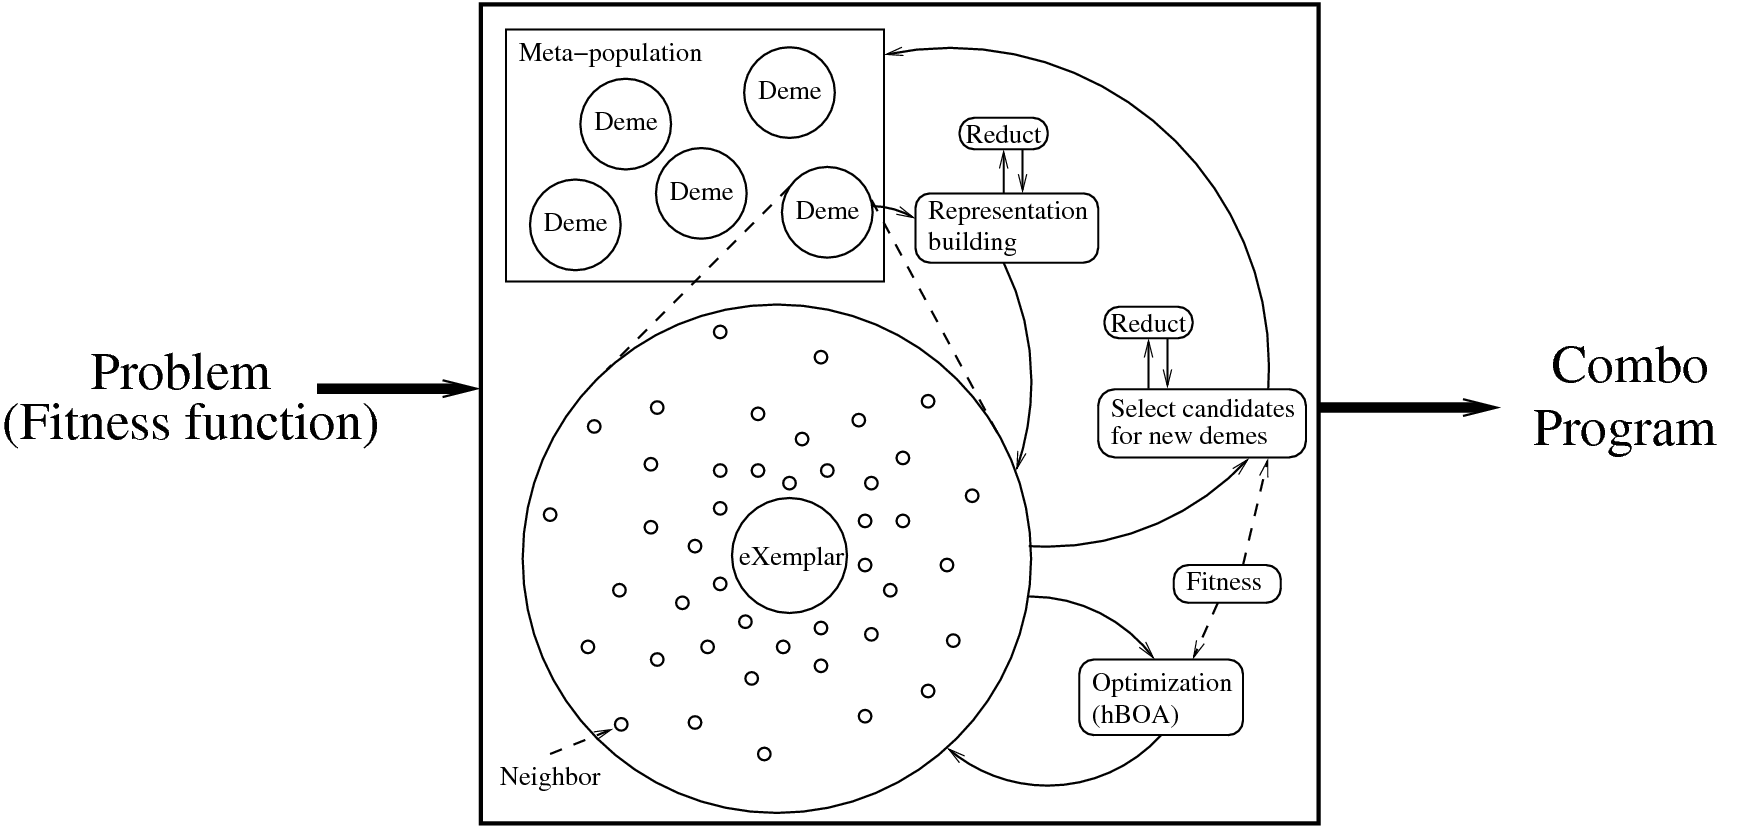
\includegraphics[scale=0.23]{images/MOSESSumDetails.png}}

\end{frame}
  
\begin{frame}
  \frametitle{What is MOSES?}

  \begin{itemize}
  \item<+-> Applications
    \begin{itemize}
    \item Genomics
    \item Sentiment Analysis
    \item Financial Prediction
    \item Virtual Agent Control
    \end{itemize}
  \item<+-> Strengths
    \begin{itemize}
    \item \alert{Compact Expressive Models}
    \item Relatively Efficient
    \end{itemize}
  \item<+-> Weaknesses
    \begin{itemize}
    \item Limited Vocabulary
    \item Limited Meta-Optimization
    \item Relatively Inefficient
    \end{itemize}
  \end{itemize}

\end{frame}

\subsection{AS-MOSES}

\begin{frame}
  \frametitle{Port MOSES to the AtomSpace}

  AS-MOSES:
  \begin{itemize}
  \item Unleash meta-optimization
  \item Expand vocabulary
  \item Fitness function versatility
  \end{itemize}

\end{frame}

\begin{frame}

  \frametitle{MOSES vs AS-MOSES}

  \begin{tabular}{ c || c | c | l}
    %% \hline
    & MOSES & AS-MOSES (now) & \\
    \hline \hline
    Description Language & Combo & Atomese & \alert{$\Rightarrow$ Expand vocabulary}\\
    \hline
    Program Space & C++ & Atomese & \alert{$\Rightarrow$ Meta-optimization}\\
    \hline
    Reduction & C++ & C++/Atomese & \alert{$\Rightarrow$ Broaden usage}\\
    \hline
    Optimization & C++ & C++ & To incorporate PLN-based EDA\\
    \hline
    Fitness Function & C++ & C++ & To support Atomese\\
    \hline
\end{tabular}

\end{frame}

\end{document}
